\documentclass[a4paper,12pt]{article}

\usepackage[utf8]{inputenc} % Kodowanie znaków
\usepackage{polski}         % Język polski
\usepackage{graphicx}       % Wstawianie obrazków
\usepackage{amsmath, amssymb} % Symbole matematyczne
\usepackage{hyperref}       % Linki w dokumencie
\usepackage{geometry}       % Ustawienia marginesów
\geometry{margin=2.5cm}     % Marginesy 2.5cm
\usepackage{indentfirst}    % Wcięcie w pierwszej linii
\usepackage{url}			 % Linkowanie w bibliografii
\usepackage{subfig}         % Wykresy
\usepackage{float}          % WYkresy

% Strona tytułowa
\title{\textbf{Aproksymacja profilu wysokościowego}}
\author{Oskar Wiśniewski, 198058\\
Politechnika Gdańska, WETI}


\begin{document}

\maketitle

\section{Wstęp}
	\subsection{Profil wysokościowy}
	Profil wysokościowy to wykres przedstawiający zmiany wartości wysokości bezwzględnej terenu w funkcji odległości od punktu początkowego trasy. Pokazuje, jak zmienia się wysokość nad poziomem morza wraz z oddalaniem się od owego punktu startowego, dzięki czemu pozwala na intuicyjnie odczytanie charakteru jakiegoś odcinka terenu.
	\par Profile wysokościowe mają szczególne znaczenie dla uczestników wyścigów kolarskich, biegaczy oraz turystów, którym to ułatwiają przygotowanie do trasy i rozplanowanie wysiłku. Korzystać z nich również mogą inżynierowie projektujący infrastrukturę transportową, geolodzy, czy architekci. 
	
	\subsection{Interpolacja}
	Interpolacja polega na wyznaczaniu przybliżonych wartości funkcji na podstawie punktów, dla których są one znane, zwanych węzłami interpolacji. Mogą nimi być przykładowo punkty pomiarowe, wyniki obliczeń numerycznych, czy punkty zadane analitycznie (na podstawie wzoru funkcji).
	\par Pierwszym etapem interpolacji jest wyznaczenie parametrów funkcji interpolacyjnej na podstawie węzłów. Następnie należy obliczyć wartości funkcji interpolacyjnej dla zadanej siatki punktów. Co istotne, z definicji interpolacja dotyczy wyłącznie oszacowania wartości wewnątrz przedziału wyznaczonego przez węzły interpolacyjne - poza zakresem mówimy o ekstrapolacji, które generalnie nie gwarantuje takiej samej dokładności jak interpolacja.
	\subsection{Interpolacja wielomianowa - metoda Lagrange'a}
	Interpolacja wielomianowa funkcji $f(x)$ polega na skonstruowaniu wielomianu $W_{N}(x)$ stopnia maksymalnie $N$ w oparciu o $N+1$ różnych węzłów interpolacyjnych $x_0, x_1, x_2, \dots, x_{N}$, dla których to zachodzi warunek:
	\begin{equation}
	W_N(x_i) = f(x_i), \quad \forall i \in \{0, 1, 2, \dots, N\}
	\end{equation}
	\par Dla danych węzłów interpolacyjnych i ich wartości można skonstruować dokładnie jeden wielomian o postaci:
	\begin{equation}
	W_N(x) = a_0 + a_1x + a_2x^2 + \dots + a_Nx^N
	\end{equation}
	\par Szczególnym przykładem interpolacji wielomianowej jest interpolacja Lagrange'a, dla której baza funkcji określona jest następującym wzorem:
	\begin{equation}
	\phi_i(x) = \prod_{j=0, j \neq i}^n \frac{(x - x_j)}{(x_i - x_j)}
	\end{equation}
	\par Po zastosowaniu go dla wszystkich węzłów interpolacyjnych można wyznaczyć wielomian interpolacyjny w następujący sposób:
	\begin{equation}
    W_N(x) = \sum_{i=0}^n f(x_i)\phi_i(x)
  	\end{equation}
  	
  	\subsection{Interpolacja funkcjami sklejanymi}
  	Interpolacja funkcjami sklejanymi (splajnami), w przeciwieństwie do wielomianowej, ma charakter lokalny, ponieważ stosuje się dla niej wielomiany niskiego stopnia między poszczególnymi węzłami. Mianowicie dla $N+1$ węzłów należy utworzyć $N$ wielomianów oznaczanych $S_0(x), S_1(x), \dots, S_{N-1}(x)$, gdzie $S_i(x)$ to funkcja sklejana dla przedziału $[x_i, x_{i+1}]$. Od ich stopnia zależy ile niewiadomych zostanie wprowadzonych i jak dokładna będzie interpolacja. W praktyce okazuje się, że wielomiany trzeciego stopnia (splajny kubiczne) pozwalają na uzyskanie dobrych aproksymacji i właśnie one zostały użyte w implementacji algorytmu. 
  	\par W celu utworzenia układu równań dla $N+1$ węzłów, wprowadzone zostały następujące założenia, z których wynikły następujące równania:
  	\begin{itemize}
  		\item Węzły są równo rozmieszczone, zatem $x_{i+1}-x_i=h, \quad \forall i \in \{0, 1, 2, \dots, N-1\}$
  		\item Szukane splajny są wielomianami trzeciego stopnia
  		\item $S_i(x_i)=f(x_i) \implies a_i = f(x_i), \quad \forall i \in \{0, 1, 2, \dots, N-1\}$
  		\item $S_i(x_{i+1})=f(x_{i+1}) \implies a_i + b_ih + c_ih^2 + d_ih^3 = f(x_{i+1}), \quad \forall i \in \{0, 1, 2, \dots, N-1\}$
  		\item $S'_{i-1}(x_i)=S'_i(x_i) \implies b_{i-1} + 2c_{i-1}h + 3d_{i-1}h^2 = b_i, \quad \forall i \in \{1, 2, \dots, N-1\}$
  		\item $S''_{i-1}(x_i)=S''_i(x_i) \implies 2c_{i-1} + 6d_{i-1}h = 2c_i, \quad \forall i \in \{1, 2, \dots, N-1\}$
  		\item $S''_0(x_0)=0 \implies c_0=0$
  		\item $S''_{N-1}(x_N)=0 \implies 2c_{N-1} + 6d_{N-1}h = 0$
  	\end{itemize}
  	\par Dzięki temu otrzymano układ równań, który łatwo można przedstawić w postaci macierzowej $\textbf{A}\textbf{x}=\textbf{b}$, gdzie \textbf{A} to macierz zawierająca wartości współczynników dla równań, \textbf{x} to wektor kolumnowy zawierający szukane współczynniki splajnów $[a_0, b_0, c_0, d_0, \dots]$, a \textbf{b} to wektor kolumnowy zawierający wartości liczbowe, np. $f(x_i)$.
  	Po znalezieniu równań splajnów postaci $S_i(x)=a_i+b_i(x-x_i)+c_i(x-x_i)^2+d_i(x-x_i)^3$ można rozpocząć aproksymację wartości dla siatki punktów. W tym celu należy odnaleźć przedział między dwoma węzłami zawierający ten punkt i podstawić go do odpowiadającemu temu przedziałowi wielomianu.
  	
	\subsection{Dane wejściowe i metodyka}
	W celu analizy różnych metod interpolacji wykorzystano profile topologiczne o różnym charakterze:
	\begin{itemize}
		\item \texttt{MountEverest.csv} - fragment profilu topologicznego dla góry Mount Everest charakteryzujący się jednym, wyraźnym wzniesieniem z maksymalną różnicą wysokości ok. 2000 m.n.p.m.
		\item \texttt{chelm.txt} - charakteryzuje się niewielkimi zmianami wysokości, z maksymalną różnicą wysokości ok. 3 m.n.p.m.
		\item \texttt{genoa\_rapallo.txt} - profil topologiczny dla trasy między Genuą a Rapallo charakteryzujący się licznymi stromymi wzniesieniami z maksymalną różnicą wysokości ok. 500 m.n.p.m.
		\item \texttt{WielkiKanionKolorado.csv} - profil topologiczny Wielkiego Kanionu charakteryzujący się pojedynczym, silnym spadkiem wysokości i maksymalną różnicą wysokości ok. 1750 m.n.p.m.
	\end{itemize}
  \begin{figure}[H]
    \centering
    \subfloat{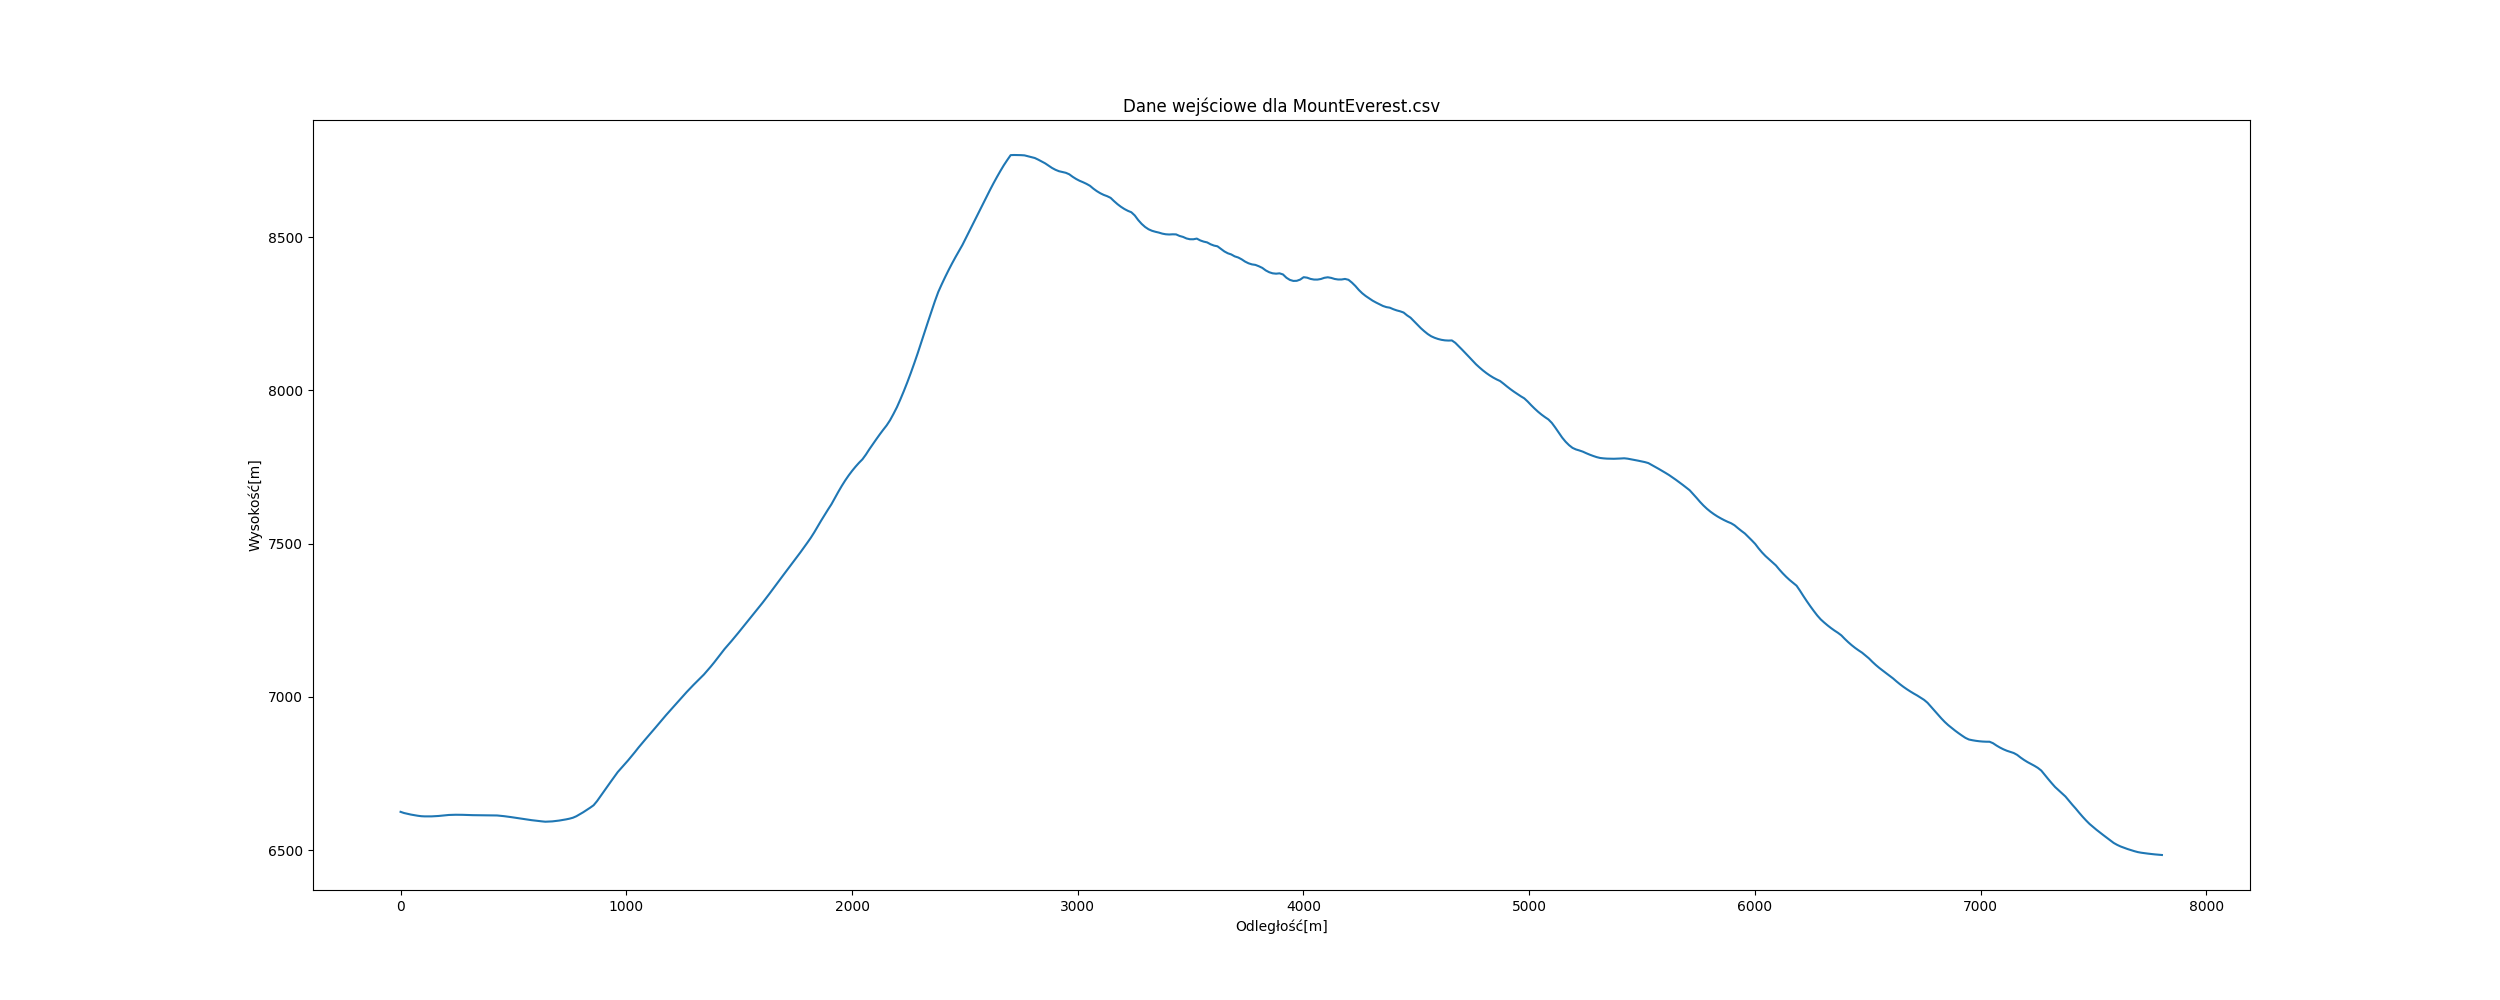
\includegraphics[width=0.5\textwidth]{../charts/input_MountEverest.png}}
    \subfloat{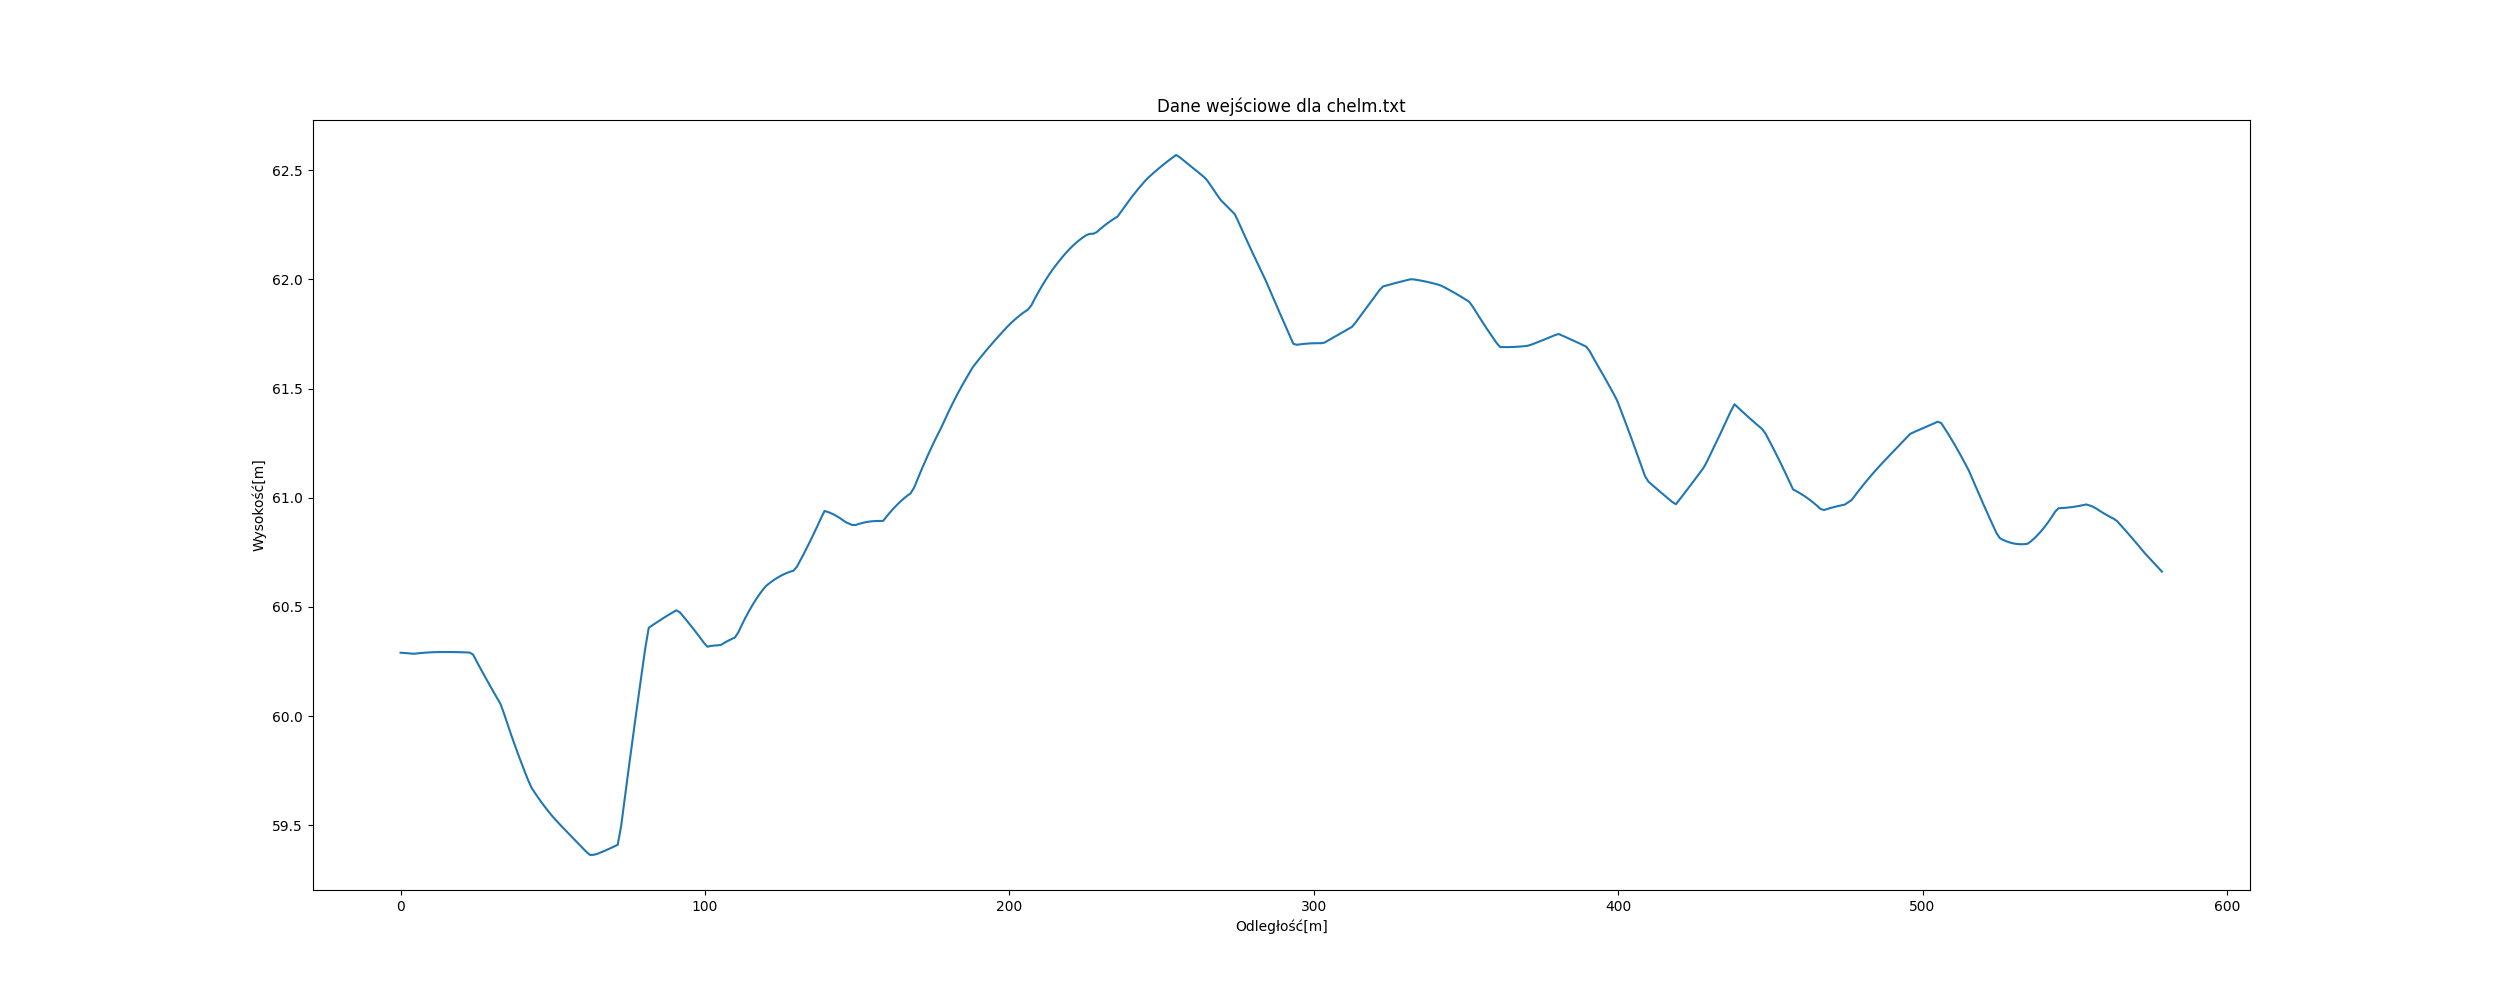
\includegraphics[width=0.5\textwidth]{../charts/input_chelm.png}}
  \end{figure}
  \begin{figure}[H]
    \centering
    \subfloat{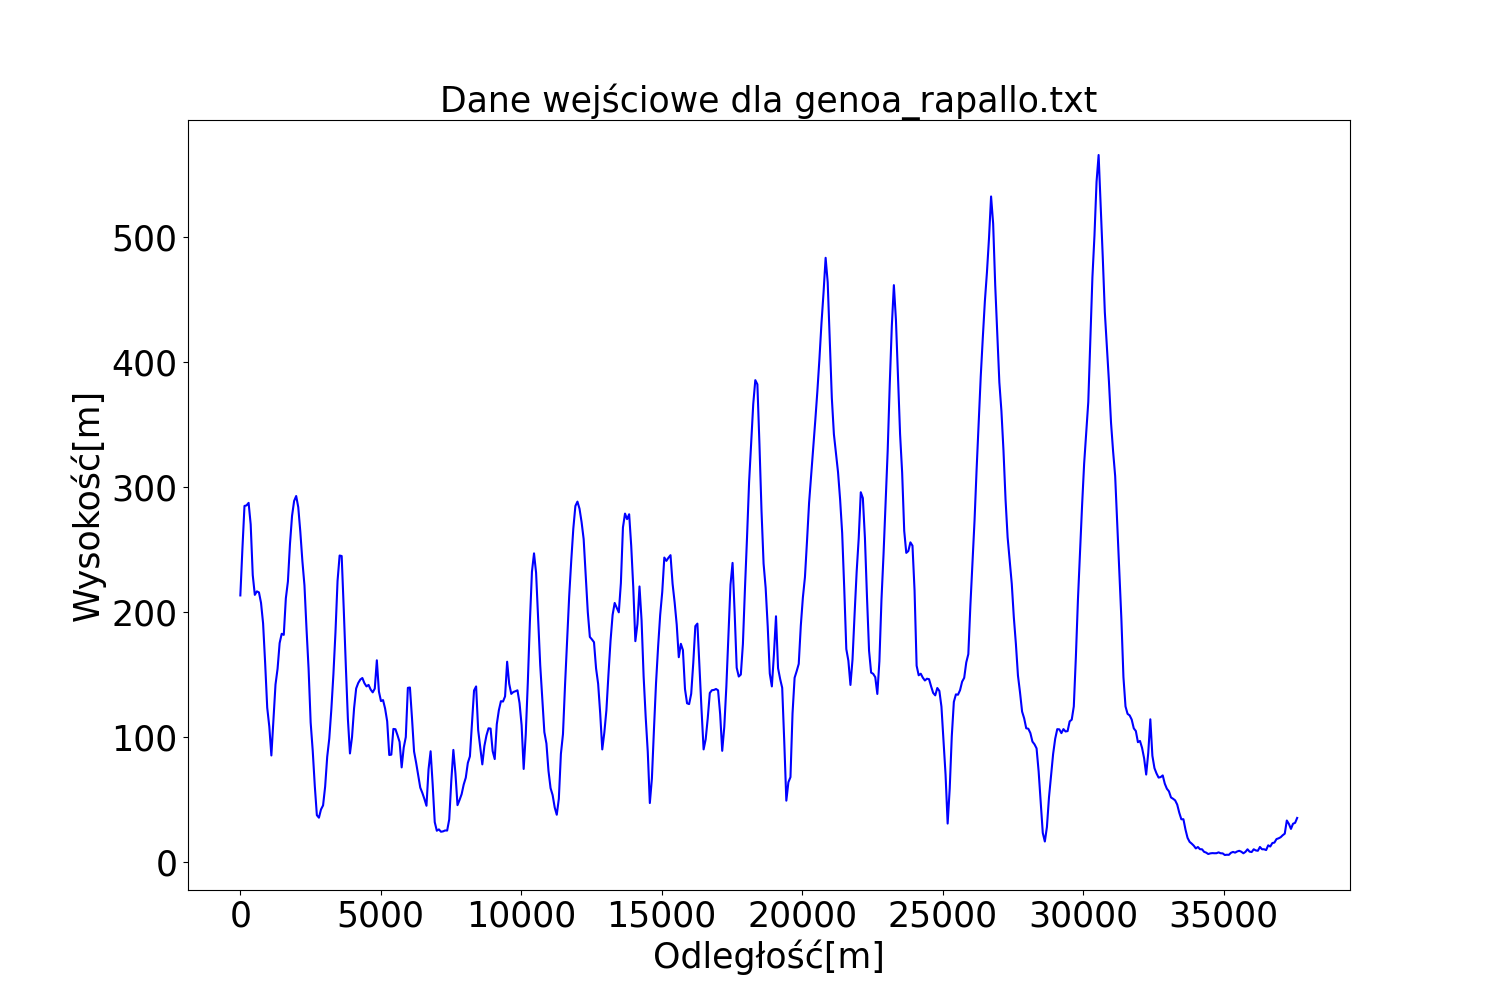
\includegraphics[width=0.5\textwidth]{../charts/input_genoa_rapallo.png}}
    \subfloat{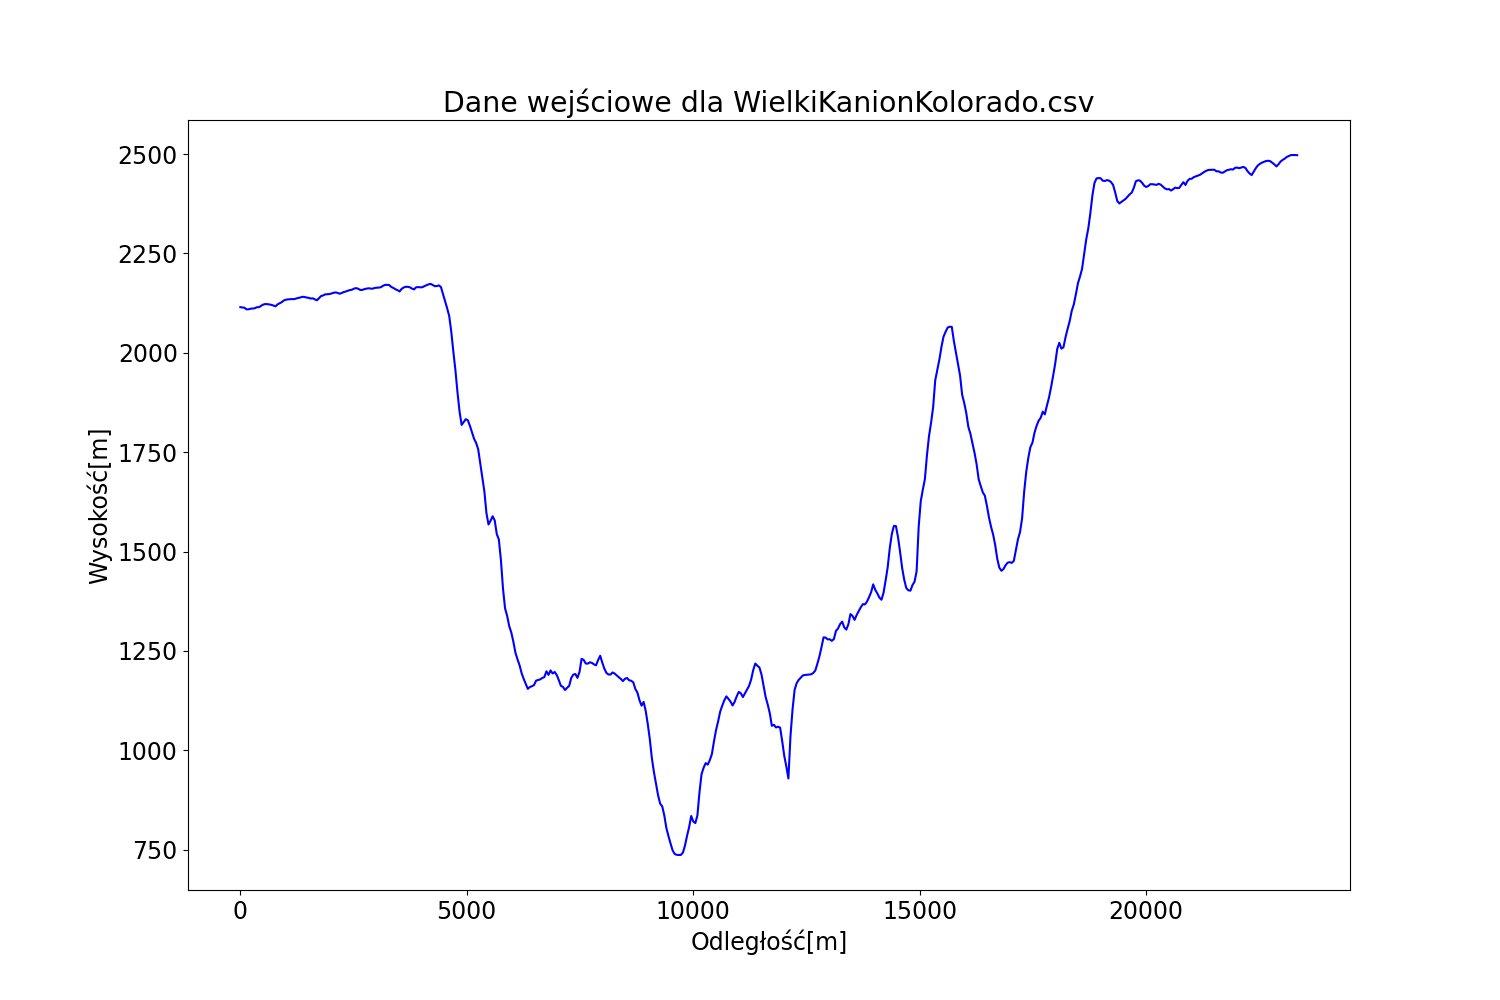
\includegraphics[width=0.5\textwidth]{../charts/input_WielkiKanionKolorado.png}}
  \end{figure}
  \par Dla każdej metody interpolacji oraz trasy wykorzystano siatkę 512 punktów, z czego jako węzły interpolacyjne wybierano kolejno 5, 10, 20 i 50 z nich. W wykresach bezpośrednio dotyczących interpolacji zastosowano skalę logarytmiczną dla lepszego zobrazowania pożądanych własności analizowanych metod.
  
\section{Analiza wyników interpolacji metodą Lagrange'a}
	W pierwszej kolejności zaimplementowano interpolację wielomianową Lagrange'a z równoodległymi węzłami interpolacyjnymi.
	
	\subsection{MountEverest.csv}
	Dla 5 węzłów wielomian stosunkowo dobrze przybliża profil topologiczny o pojedynczym wzniesieniu. Jednak dla coraz większej ilości węzłów można zauważyć, że wzrastającej dokładności aproksymacji w środku przedziału towarzyszy coraz to silniejsza niedokładność na jego skraju. Niedokładność ta pokrywa coraz to większy przedział i błąd przybliżenia staje się coraz większy - dla 50 węzłów wartość jest rzędu $10^12$ zamiast wzorcowej ok. 7000. Efekt ten nazywany jest efektem Rungego i omawiany będzie szerzej w dalszej części opracowania.
	\begin{center}
        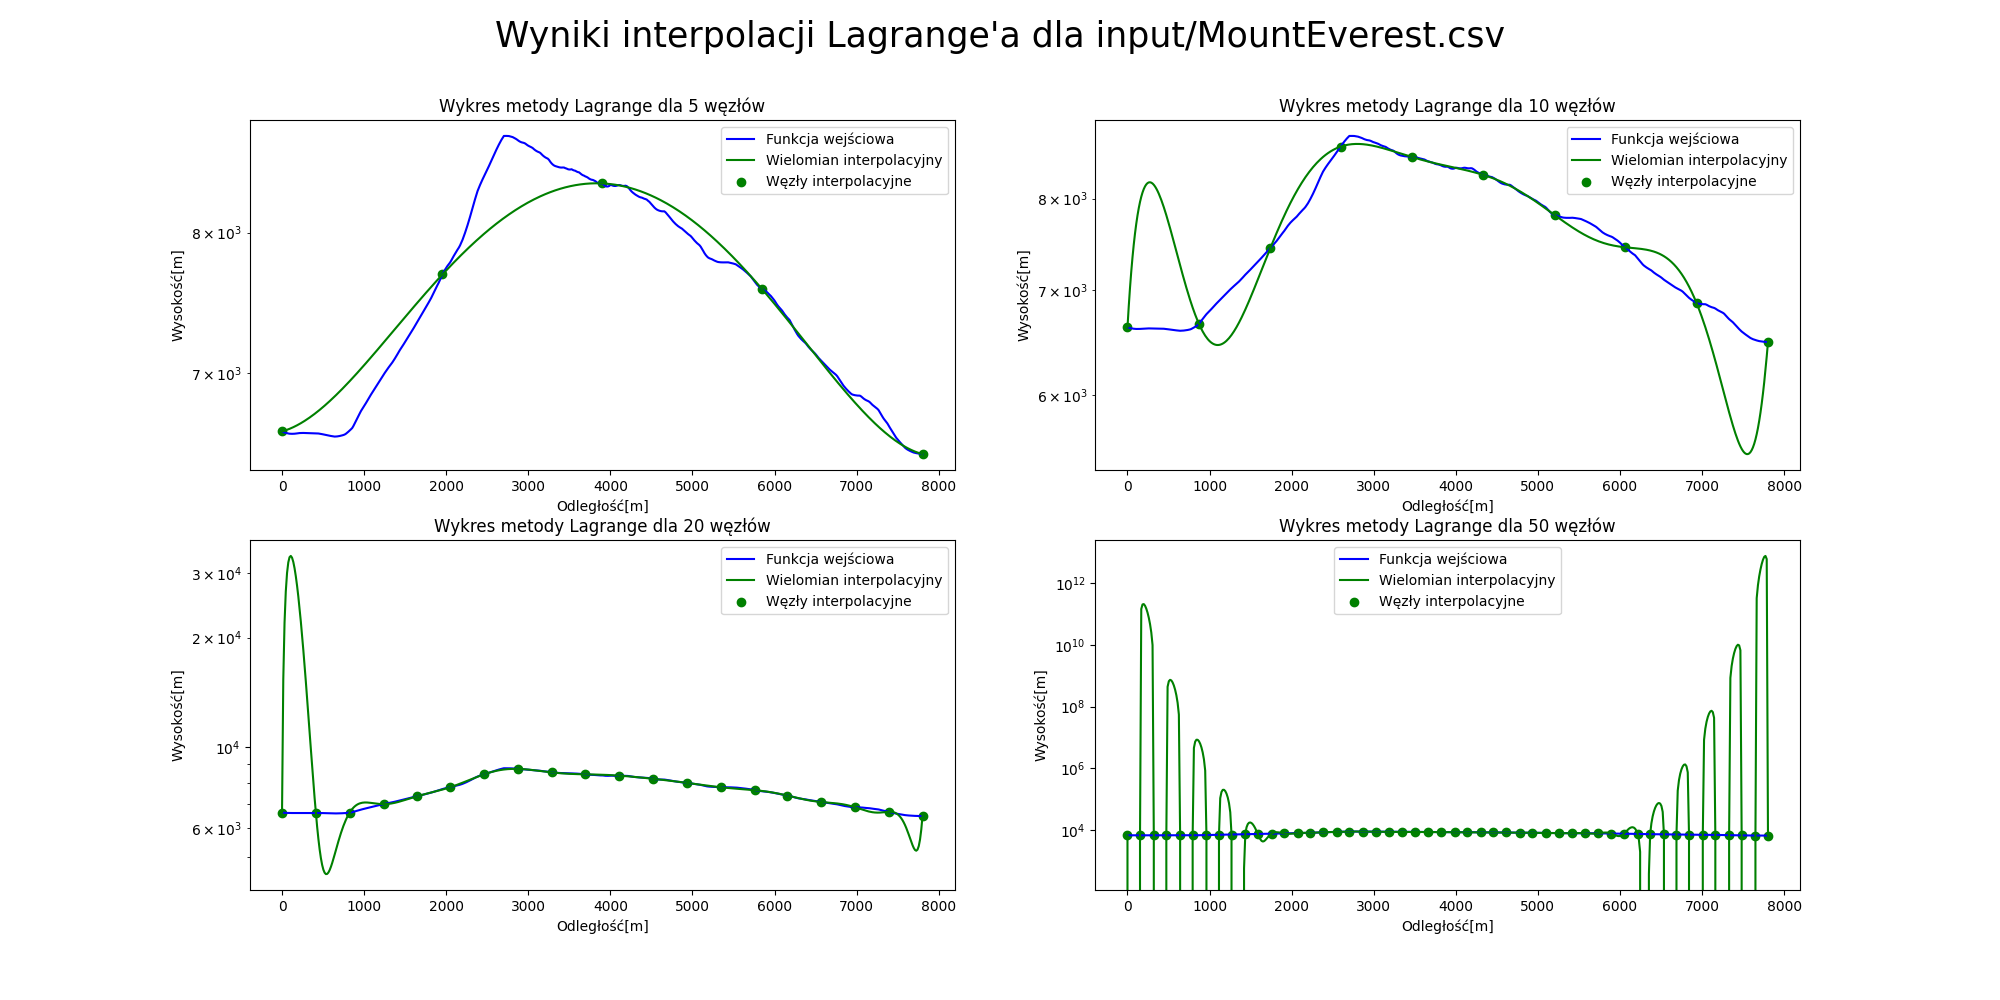
\includegraphics[scale=0.4]{../charts/lagrange_MountEverest.png}
    \end{center}
	
	\newpage
	\subsection{Chelm.txt}
	Dla w przybliżeniu stałego profilu topologicznego 5 węzłów z grubsza go aproksymuje, omijając drobne zmiany wysokości. Ponownie, dla większej liczby węzłów można zaobserwować coraz silniejszy efekt Rungego.
	\begin{center}
        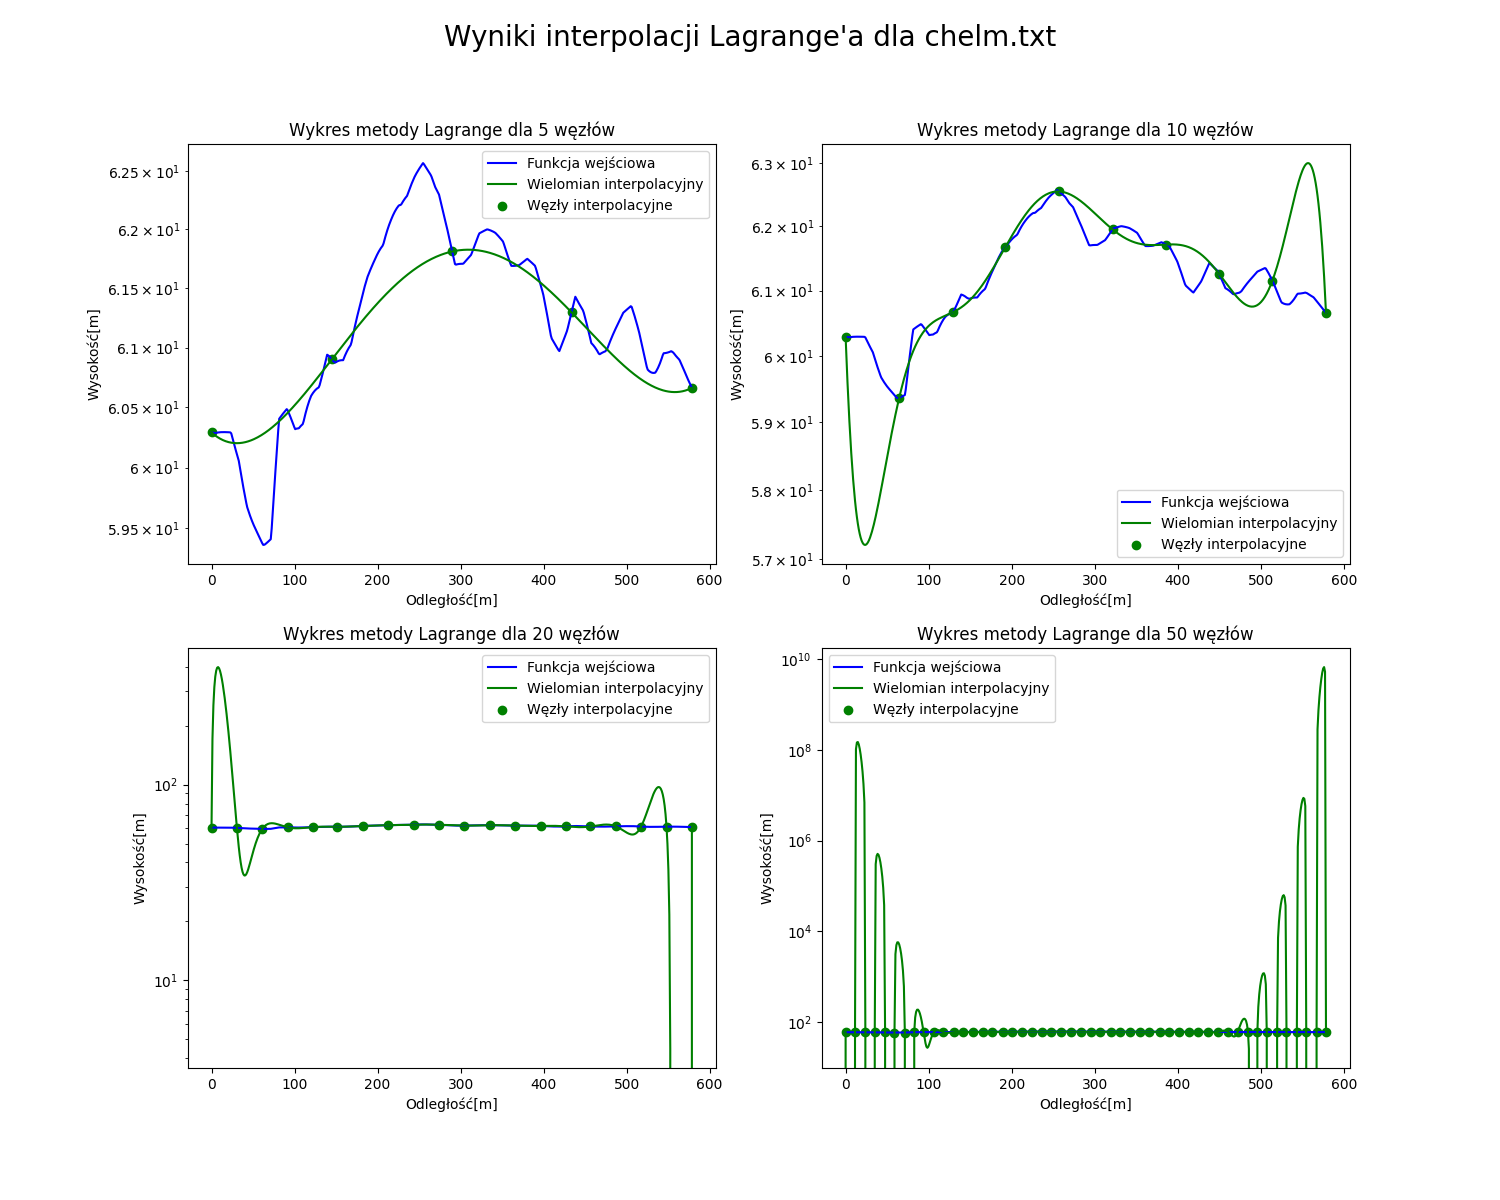
\includegraphics[scale=0.4]{../charts/lagrange_chelm.png}
    \end{center}
    
    \newpage
   	\subsection{Genoa\_rapallo.txt}
	Dla profilu topologicznego o silnych oscylacjach w żadnych przypadku nie udało się dobrze go przybliżyć. Dla 5 węzłów wielomian zarysowuje jedynie trend funkcji, a dla 10 węzłów przy silniejszej zmianie wysokości następuję gwałtowna zmiana wartości funkcji interpolującej z nieakceptowalnym błędem aproksymacji. Z kolei dla 20 i 50 węzłów ponownie zaobserwowano efekt Rungego, w ostatnim przypadku na jeszcze większej części przedziału niż przedtem.
	\begin{center}
        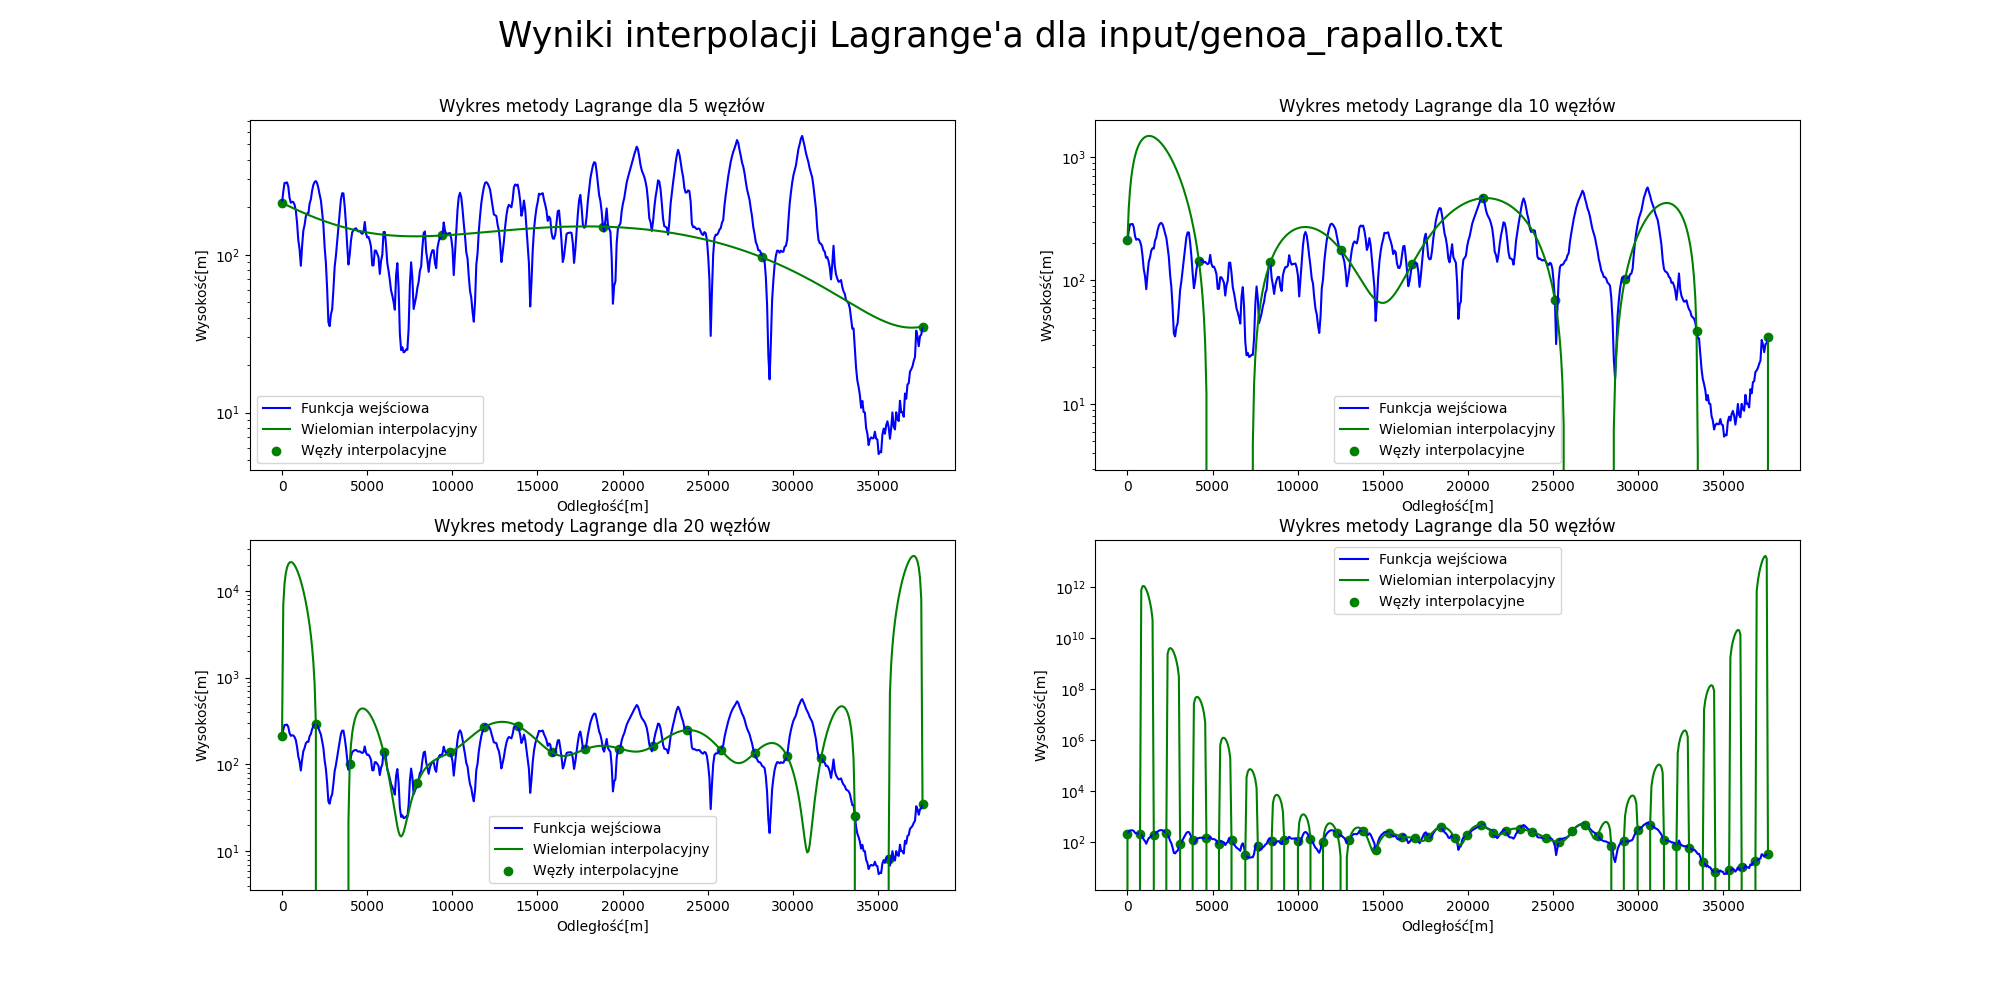
\includegraphics[scale=0.4]{../charts/lagrange_genoa_rapallo.png}
    \end{center}
    
    \newpage
	\subsection{WielkiKanionKolorado.txt}
	Dla profilu topologicznego o silnym spadku dokładność aproksymacji jest podobna do tej dla wzniesienia. Różnicę zaobserwowano dla 20 i 50 węzłów, gdzie wystąpił silniejszy efekt Rungego.
	\begin{center}
        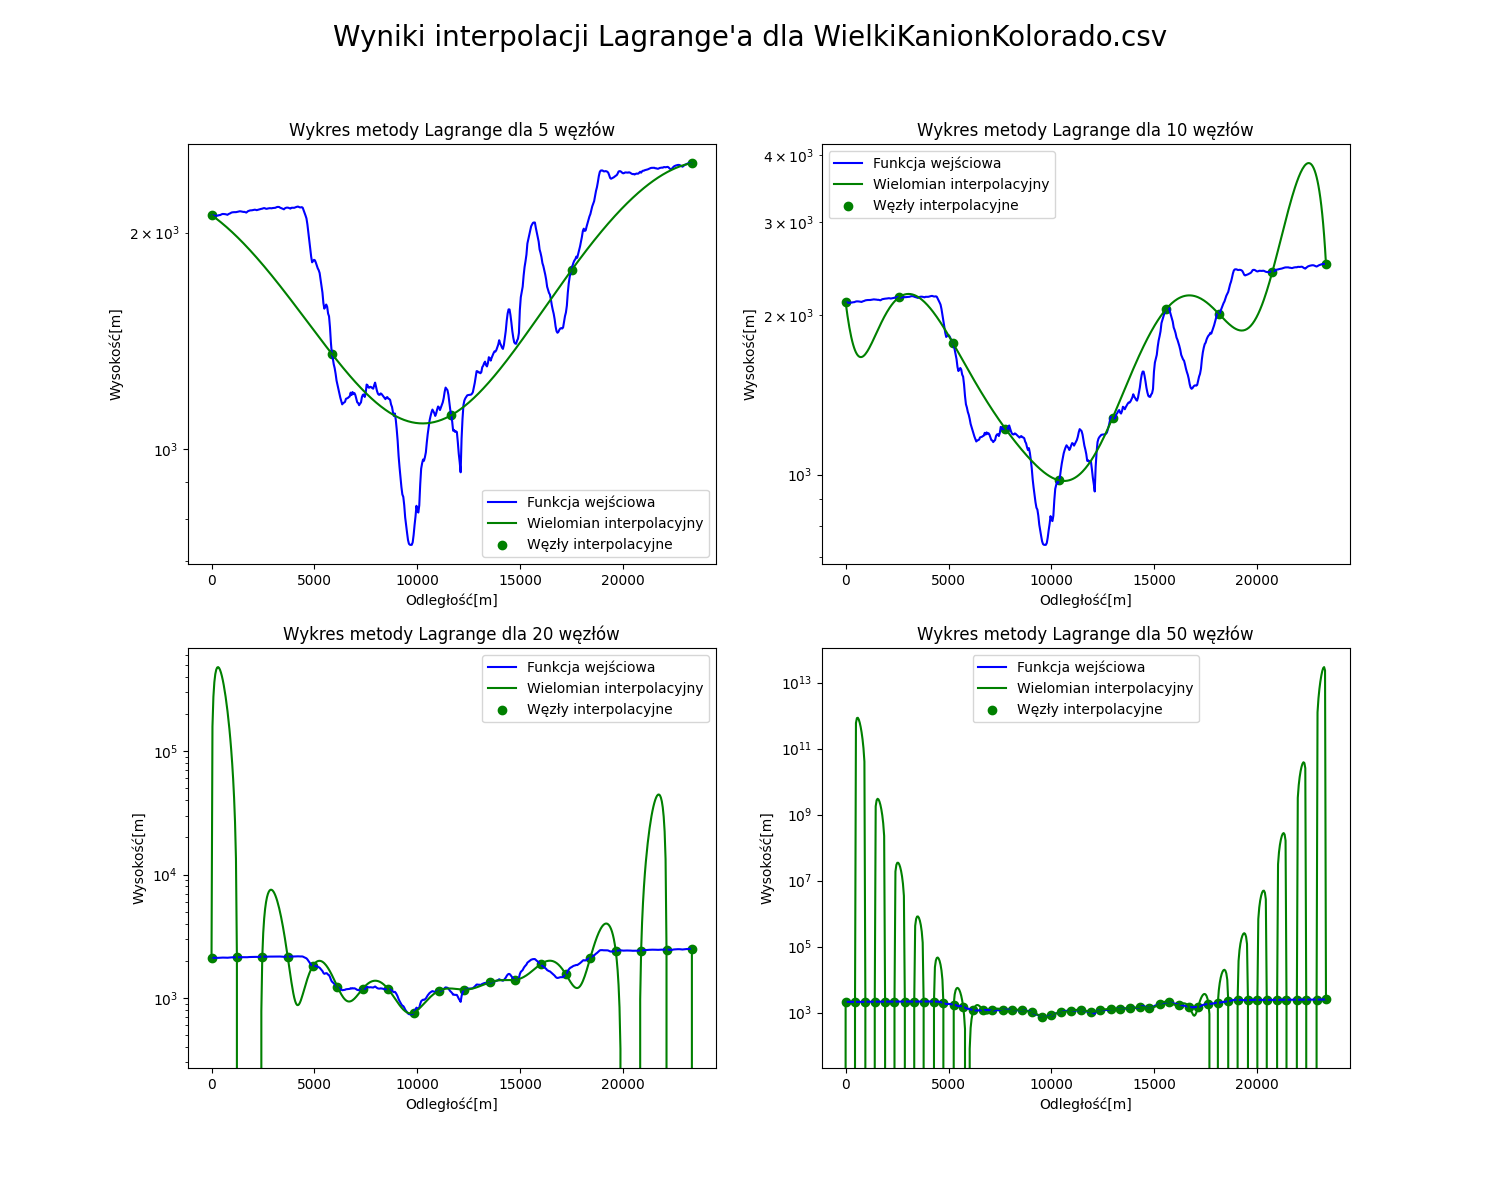
\includegraphics[scale=0.4]{../charts/lagrange_WielkiKanionKolorado.png}
    \end{center}
    
\section{Analiza wyników interpolacji metodą Lagrange'a z węzłami Czebyszewa}
	Jedną z metod poprawy dokładności interpolacji wielomianowej jest zmiana sposoby rozmieszczenia węzłów interpolacyjnych. Przykładem są węzły Czebyszewa drugiego rodzaju definiowane następująco na przedziale $[a, b]$:
	\begin{equation}
	x_i = \frac{a+b}{2} + \frac{b-a}{2}\cos(\frac{i}{N-1}\pi), \quad \forall i \in \{0, 1, 2, \dots, N-1\}
	\end{equation}

\end{document}